\documentclass[12pt]{article}
\usepackage[spanish]{babel}
\usepackage[utf8]{inputenc}
\usepackage{amsmath}
\usepackage{listings}
\usepackage[usenames]{color}
\definecolor{gray97}{gray}{.97}
\definecolor{gray75}{gray}{.75}
\definecolor{gray45}{gray}{.45}
\definecolor{azul1}{RGB}{141,198,163}
\definecolor{azul2}{RGB}{24,107,122}
\definecolor{verde1}{RGB}{44,186,34}

\usepackage{textcomp}
\lstset{
		frame=Ltb,
		framerule=1pt,
		framextopmargin=3pt,
		framexbottommargin=3pt,
		framexleftmargin=0.4cm,
		framesep=0pt,
		rulesep=.4pt,
		backgroundcolor=\color{gray97},
		rulesepcolor=,
        tabsize=4,
        rulecolor=\color{azul1},
        basicstyle=\scriptsize\rmfamily,
        upquote=true,
        aboveskip={1.5\baselineskip},
        columns=fixed,
        showstringspaces=false,
        extendedchars=true,
        breaklines=true,
        prebreak = \raisebox{0ex}[0ex][0ex]{\ensuremath{\hookleftarrow}},
        showtabs=false,
        showspaces=false,
        showstringspaces=false,
        identifierstyle=\rmfamily,
        keywordstyle=\color[rgb]{0,0,1},
        commentstyle=\color[rgb]{0.133,0.545,0.133},
        stringstyle=\color[rgb]{0.627,0.126,0.941},
        keywordstyle=\bfseries,
        %
		numbers=left,
		numbersep=15pt,
		numberstyle=\tiny,
		numberfirstline = false,
		breaklines=true,
		}
\usepackage{graphicx}
\usepackage[colorinlistoftodos]{todonotes}
\usepackage{natbib} %citas bibliograficas estilo APA :p
\usepackage{eso-pic}
\usepackage{avant}
\usepackage[top=2cm,bottom=2cm,left=2.5cm,right=3cm,headsep=8pt,a4paper]{geometry}
\usepackage{fancyhdr}
\pagestyle{fancy}
\fancyhf{}
%\fancyhead[LE,RO]{}
\fancyhead[RE,LO]{Procesamiento de Señales II}
\fancyfoot[CE,CO]{\leftmark}
\fancyfoot[LE,RO]{\thepage}
\renewcommand{\headrulewidth}{2pt}
\renewcommand{\footrulewidth}{1pt}
\usepackage{tabu}
\usepackage{array}
\usepackage{multirow}
\usepackage{amssymb}
\usepackage{makeidx}
\graphicspath{ {images/} }
\usepackage{wrapfig}
\usepackage{enumerate}
\usepackage{amsmath,tikz}
\usetikzlibrary{matrix}
\usepackage{steinmetz}
\newcommand*{\horzbar}{\rule[0.05ex]{2.5ex}{0.5pt}}
\usepackage{calc}
\date{\today}


\begin{document}

\begin{titlepage}
\newcommand{\HRule}{\rule{\linewidth}{0.5mm}} 
\center
\textsc{\LARGE  Benemérita Universidad \\[0.2cm] Autónoma de Puebla}\\[1.5cm] 

\includegraphics[width=4cm]{imagenes/escudo.jpg}\\[1cm]
\textsc{\Large Facultad de Ciencias de la Electrónica}\\[0.5cm] 
\textsc{\large Licenciatura en Electrónica}\\[0.5cm]
\HRule \\[0.4cm]
{ \huge \bfseries Práctica 2}\\[0.4cm] 
\HRule \\[1.5cm]
\begin{minipage}{\textwidth}
\center 

\emph{Profesor:} \\
Fernando López Marcos \\[1cm]

\begin{tabular}{ll}
\emph{Alumnos:} & \emph{Número de Matrícula:}\\
Hanan Ronaldo Quispe Condori  & 555010653 \\
Erick Sandro Niño García & 201631150\\
Carlos Alfredo Vega Aguilar & 201632131 \\
\end{tabular}
\end{minipage}\\[2cm]
\today
\end{titlepage}

%\newpage
%~\vfill
%\thispagestyle{empty}
%\begin{figure}[hbtp]


%\includegraphics[width=4cm]{IMAGENES/motordc}
%\end{figure}
%\noindent \textsc{Trabajo Encargado: Problemas en MatLab \\ Máquinas Eléctricas \\ Universidad Nacional de San Antonio abad del Cusco}\\
%noindent \textsc{Ingeniería Electrónica }\\
%\noindent \textit{Tercera revisión, \today}

%\tableofcontents indice bloqueado xD

\newpage

\section{Introducción}
Se realiza un filtro digital mediante fdatool de matlab y el entorno de matlab. El filtro es de ventana Blackman=1, fc= 440 Hz, banda  de  transición  de 30\%  de  la  frecuencia central, una atenuación mínima de 15dB en banda de rechazo, un rizado en banda de paso máximo de 2 dB y una frecuencia de muestreo de 44100 Hz.

\section{Objetivos}
Que el alumno utilice la herramienta fdatool para la implementación de un filtro digital FIR.
\section{Desarrollo}
De acuerdo a los requerimientos planteados anteriormente, se comienza ejecutando fdatool para analizar qué otros datos son necesarios para realizar el diseño del filtro: 
\\
  \begin{figure}[h]
        \centering
        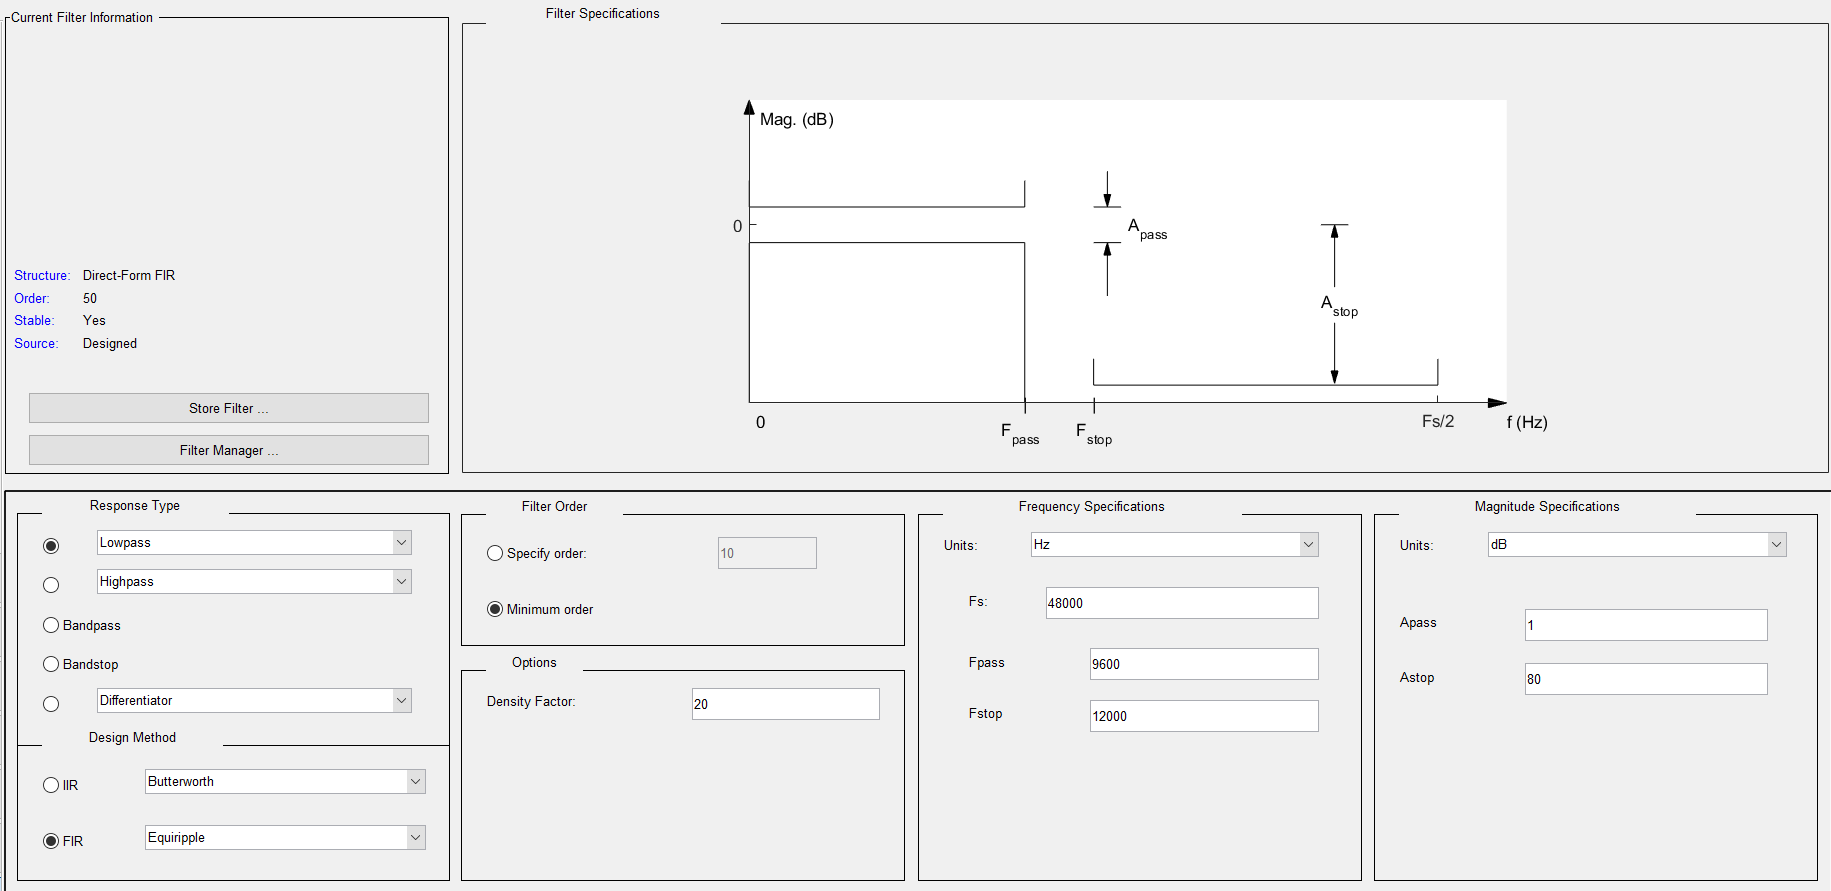
\includegraphics[width=14cm, height=6cm]{imagenes/fdatool.png}
        \caption{Vista a la ventana de fdatool.}
    \end{figure}
    \\
Se observa que se requieren datos como el tipo de filtro (LP, HP, BP...), método de diseño (FIR, IIR), orden del filtro, frecuencia de corte y de muestreo, entre otros. De todos estos parámetros, lo único que se desconoce es el orden del filtro, por lo que se calcula a partir de la siguiente ecuación característica de la ventana Blackman:
\begin{equation}
    \Delta f = \dfrac{5.5}{N}
\end{equation}

Donde N es el orden del filtro, y $\Delta f$ está definido como:
\begin{equation}
    \Delta f = \dfrac{f_{c}}{f_{m}} = \dfrac{440}{44100} = 0.0099
\end{equation}
Entonces despejando a (1):
\begin{equation}
    N = \dfrac{5.5}{0.0099} = 555
\end{equation}
Obteniendo así el dato faltante, con esto se procede a llenar el formulario y a diseñar el filtro para obtener sus coeficientes y comprobar su funcionamiento:
\\
  \begin{figure}[h]
        \centering
        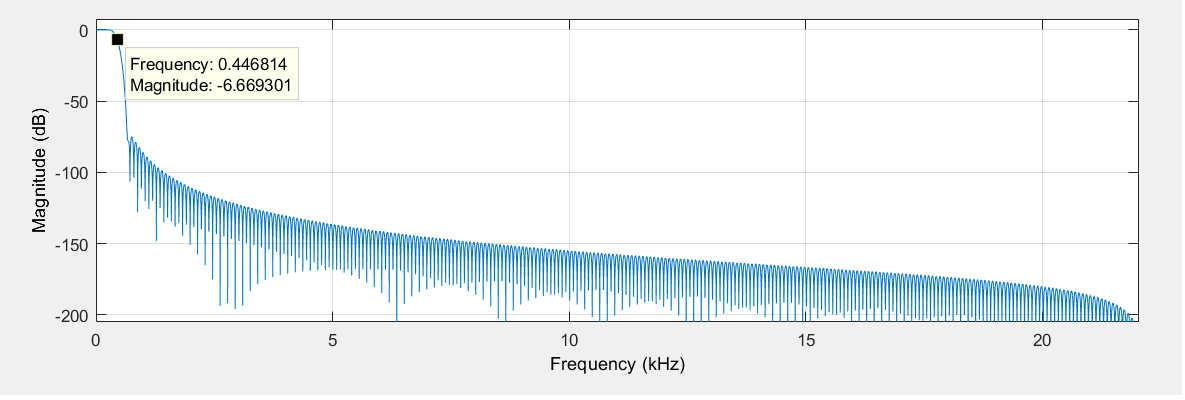
\includegraphics[width=14cm, height=6cm]{imagenes/resp_magn.png}
        \caption{Respuesta en magnitud del filtro según fdatool.}
    \end{figure}
    \\
En la figura 2 se observa que para una frecuencia muy cercana a $f_{s}$ la atenuación llega a más de -6dB, una cifra satisfactoria. 
\\
Poniendo a prueba el filtro en un programa de MATLAB proporcionado por el profesor, se colocan 2 valores diferentes en la variable que corresponde a la frecuencia de la señal que será pasada por el filtro: 440Hz y 572Hz. Esta última cifra corresponde al treinta por ciento de banda de transición que requiere cumplir el filtro. Se obtuvo lo siguiente
  \begin{figure}[h]
        \centering
        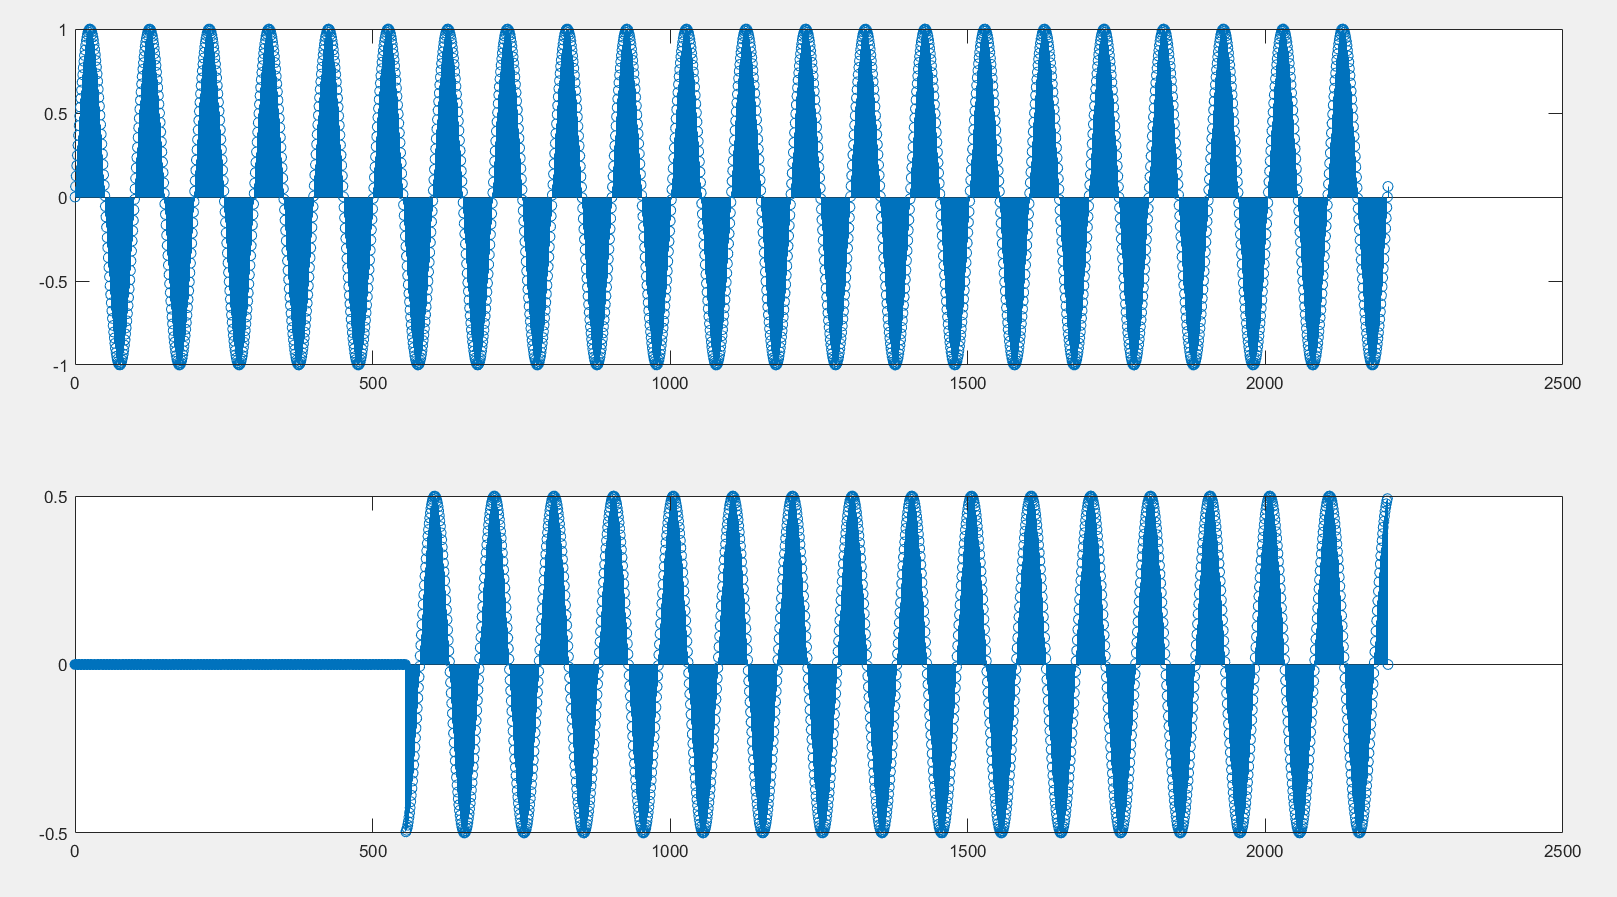
\includegraphics[width=14cm, height=5cm]{imagenes/respFIR_440.png}
        \caption{Señal de 440Hz procesada por el filtro.}
    \end{figure}
Como se observa en la figura 3, con la señal a una frecuencia igual a la de corte del filtro, se llega a una amplitud aproximada de 0.5, que en dB es equivalente a 6dB, por lo que se comprueba su excelente atenuación.
\vspace{80mm}
\begin{figure}[h]
    \centering
    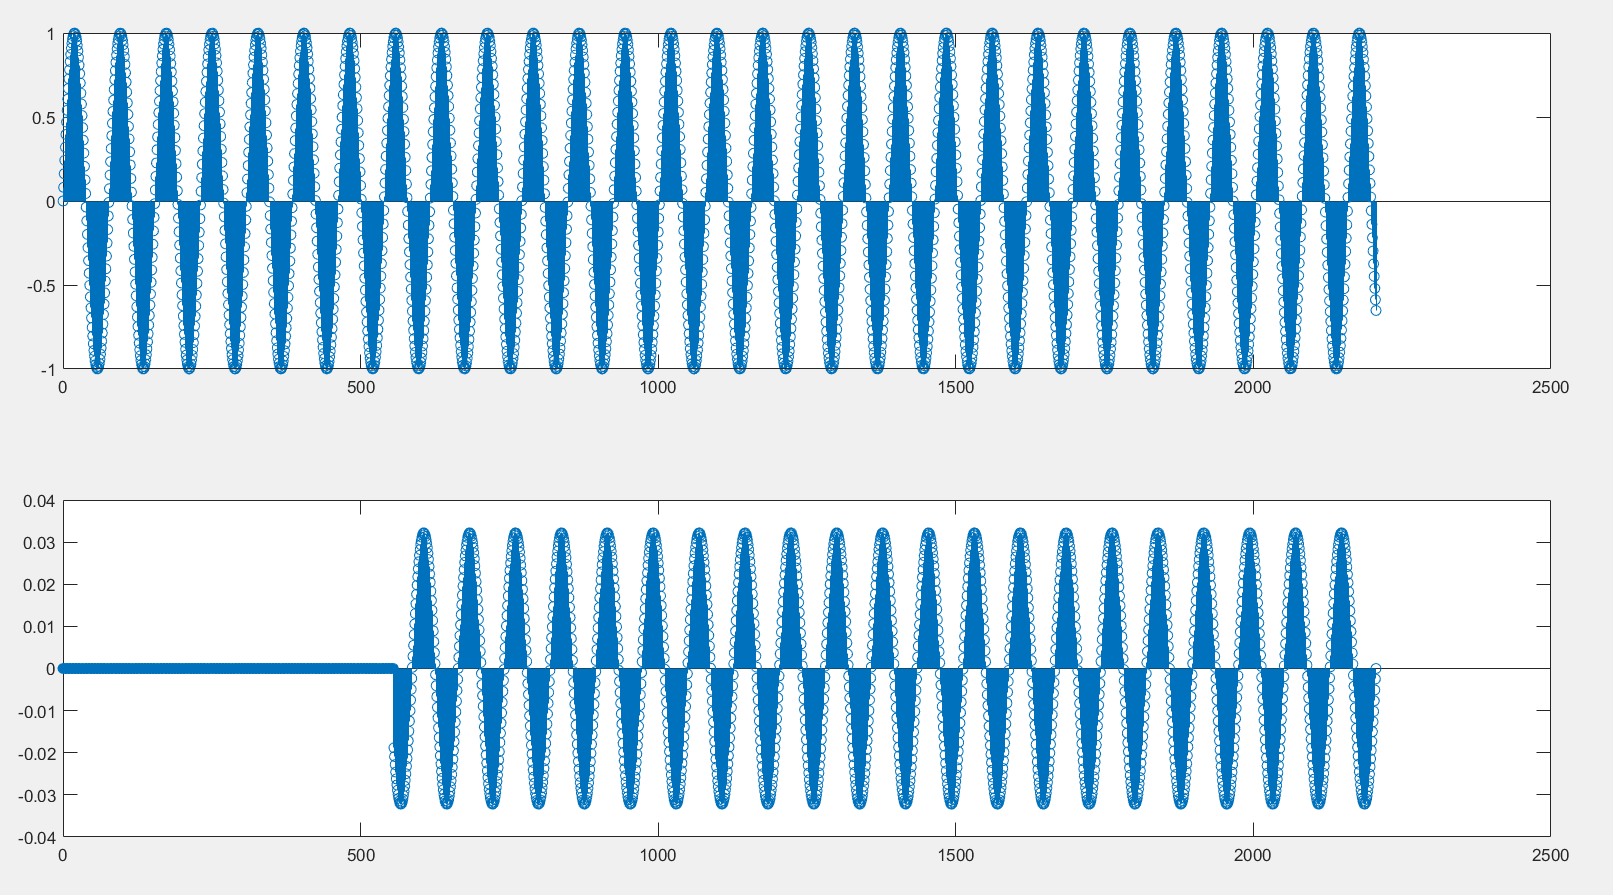
\includegraphics[width=14cm,height=5cm]{imagenes/respFIR_572.png}
    \caption{Señal de 572Hz procesada por el filtro.}
\end{figure}

En la figura 4 se puede notar que, a una frecuencia treinta porciento mayor a la central del filtro, se obtiene una atenuación excelente (aprox 30dB), superior a los 15dB que era el mínimo a lograr, por lo que se comprueba el correcto funcionamiento del filtro.
\section{Conclusiones}
\begin{itemize}
    \item Se puede comprobar que la linealidad de fase del filtro diseñado es de tipo 2, los coeficientes del filtro que nos da la herramienta de $fdatool$ de MATLAB al ser nuestro filtro del tipo FIR son los valores de la respuesta al impulso, conocido esto en \cite{deergha2018digital} se menciona que estos filtros se pueden clasificar en simétricos y antisimetricos segun sea la cantidad de coeficientes $N$ par en el primer caso e impar en el segundo caso, en nuestro caso este numero de muestras es $556$ corresponde al caso simétrico, esta respuesta al impulso cumplira la siguiente ecuación.
    \begin{equation}
        \begin{split}
           h(n)&=h(N-n), 0\le n \le N \\ 
        \end{split}
        \label{eq:filter}
    \end{equation}
    Usando MATLAB podemos comparar los valores de este vector usando el siguiente script, dando como resultado un vector de booleanos siendo cada uno de estos la comparación de los elementos según la ecuación \ref{eq:filter}.
    \lstinputlisting[language=Matlab]{matlab/testing.m}
    Este script da como resultado un vector de booleanos donde todos los elementos corresponden al estado $True$.
    Tambien esto se puede observar gráficamente. 
\vspace{150mm}
    \begin{figure}[h]
        \centering
        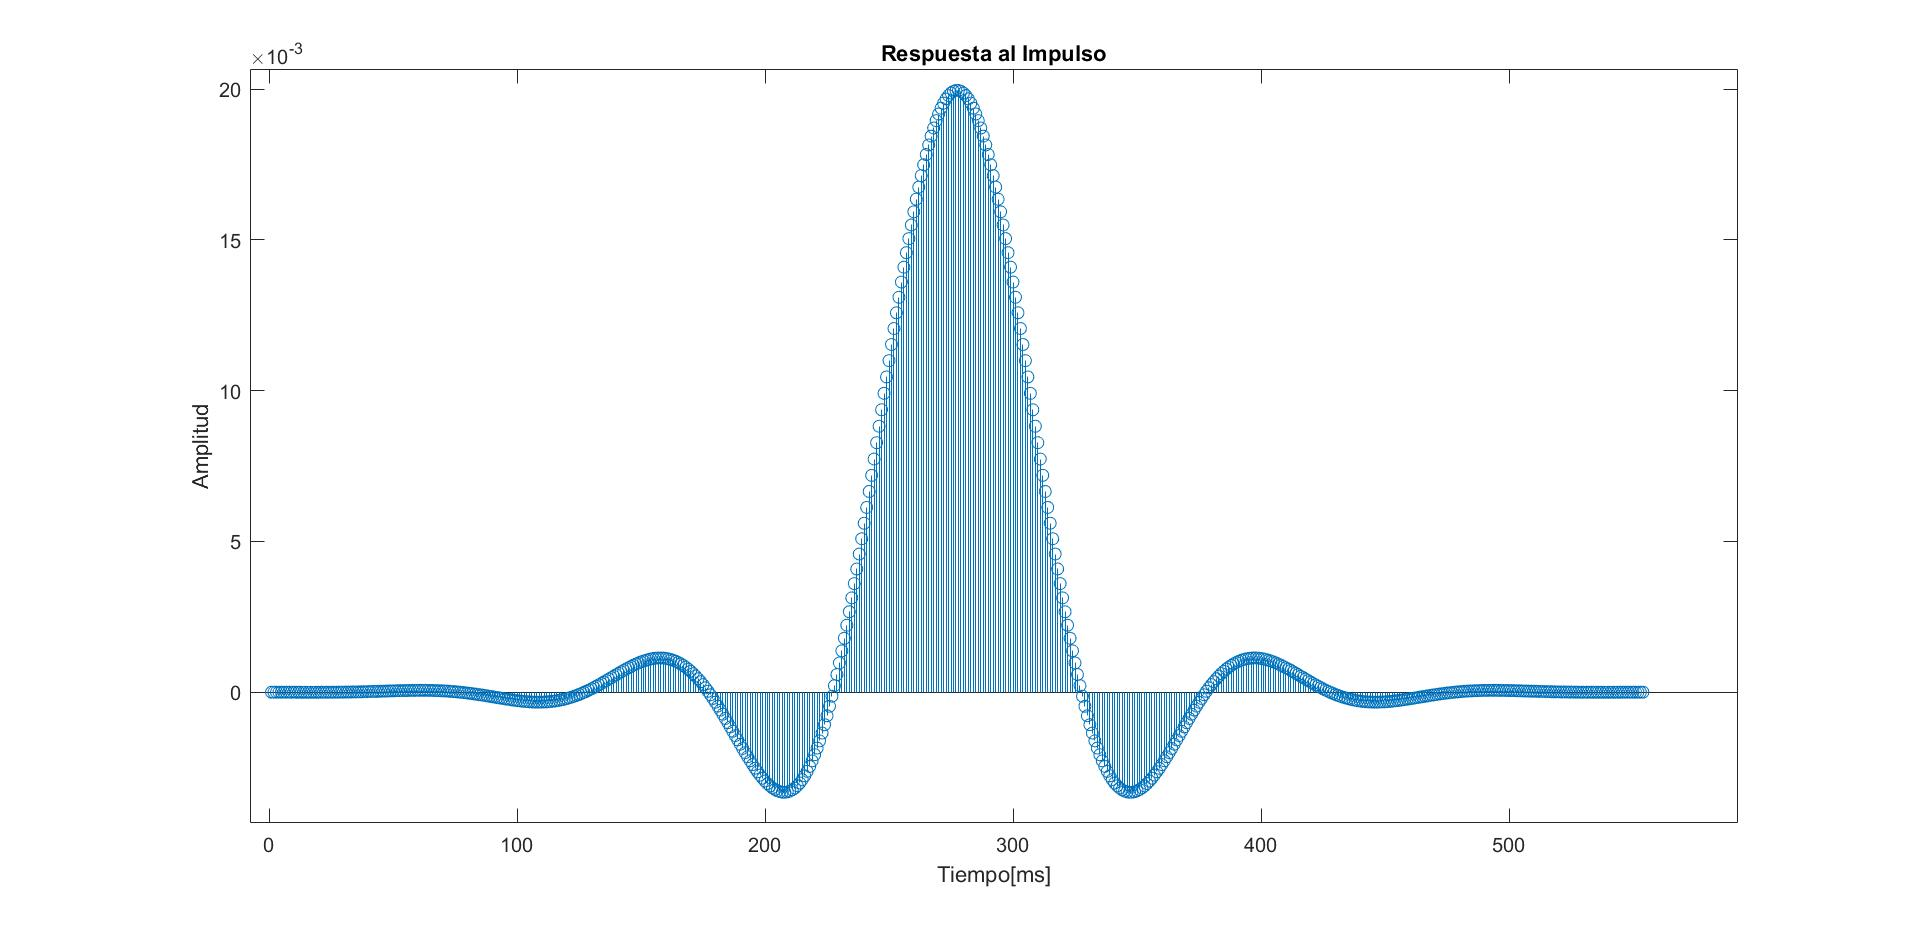
\includegraphics[width=16cm, height=6cm]{imagenes/impulse.jpg}
        \caption{Respuesta al Impulso del Filtro FIR Diseñado.}
    \end{figure}
    \item Se hara una comparación entre las respuestas en frecuencia cuando el orden del filtro aumenta, se muestra a continuación la respuesta para un orden de $48$ y de orden $555$.
    \begin{figure}[h]
        \centering
        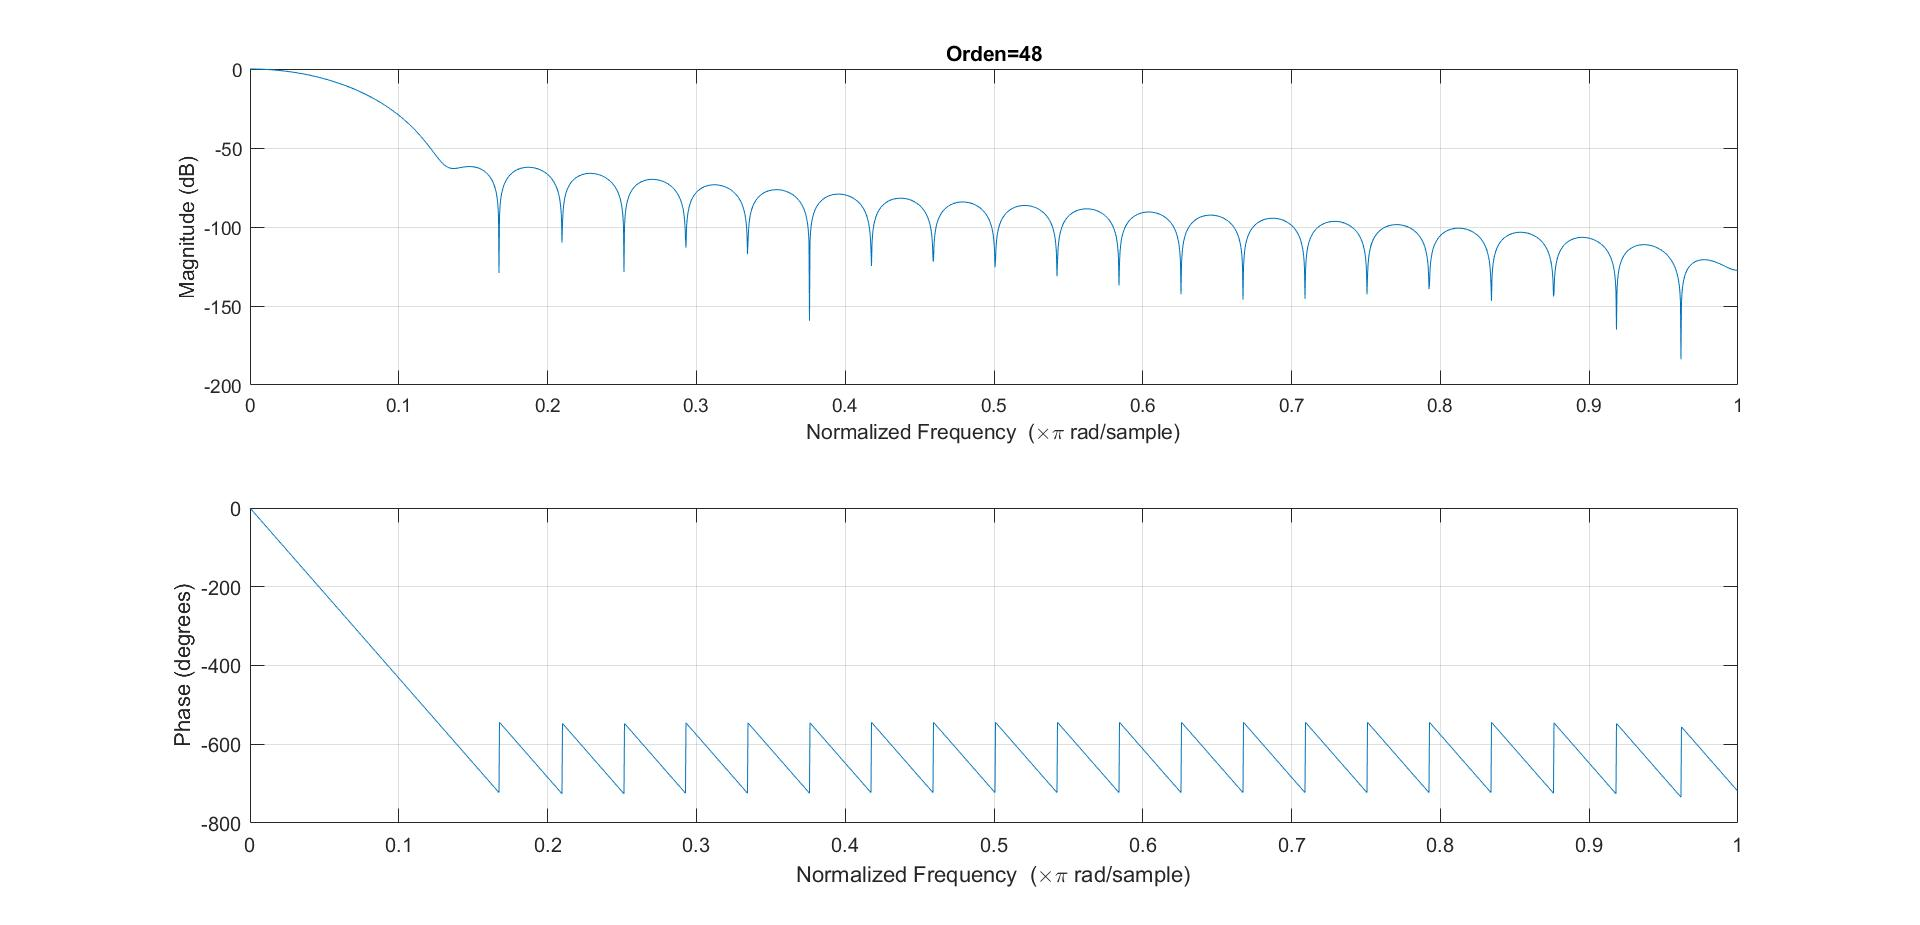
\includegraphics[width=14cm, height=4cm]{imagenes/Order48.jpg}
        \caption{Respuesta en Frecuencia Orden 48.}
    \end{figure}
    %\vspace{80mm}
    \begin{figure}[h]
        \centering
        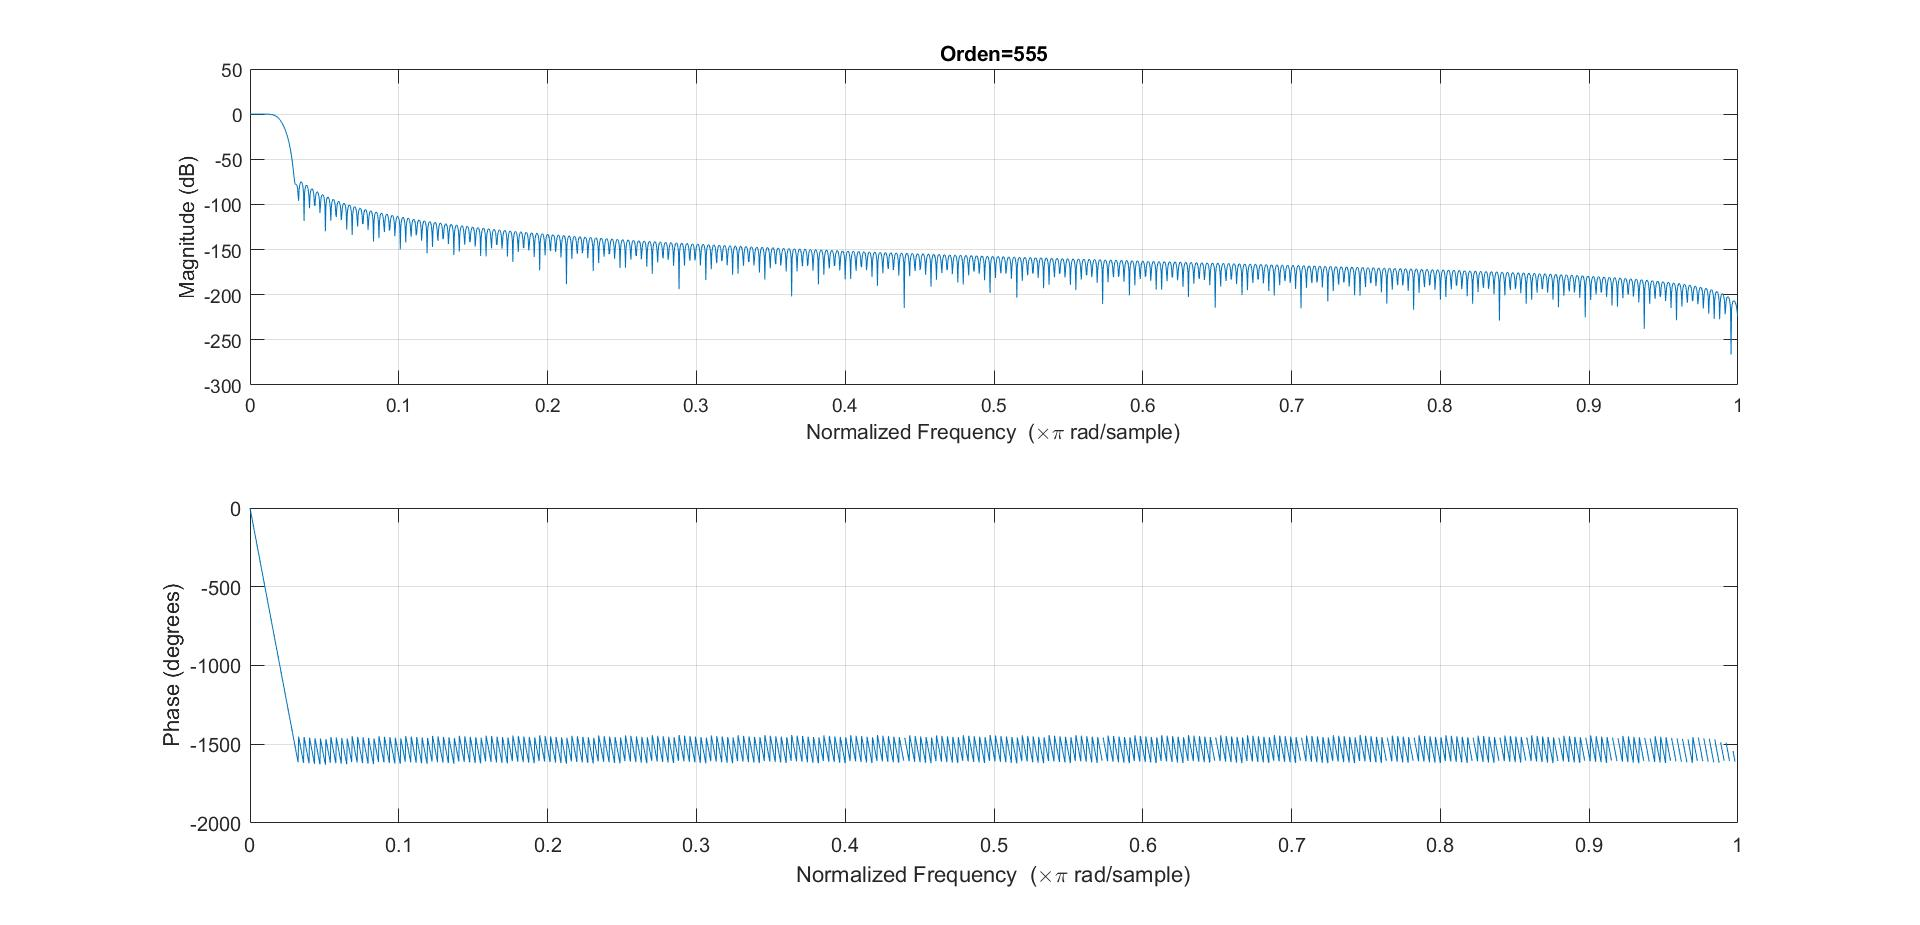
\includegraphics[width=14cm, height=4cm]{imagenes/Order555.jpg}
        \caption{Respuesta en Frecuencia Orden 555.}
    \end{figure}

    Podemos observar que ambas tienen una respuesta en frecuencia similar, variando esta en la magnitud del desfase presente en altas frecuencias. 
    \item El orden del filtro fue calculado mediante la aproximación dada en \cite{ifeachor2002digital} este orden alto es una caracteristica de los filtros $FIR$ estos filtros se pueden diseñar para una fase lineal pero necesitan de un orden alto en comparacion de los filtros IIR.
    \end{itemize}
    
\bibliographystyle{ieeetr}
\bibliography{biblio}
\section{Apéndice: Códigos.}
\lstinputlisting[language=Matlab]{matlab/FIR_Equipo2.m}
\end{document}

